%  IR_Design.tex
%  Document created by seblovett on seblovett-Ubuntu
%  Date created: Thu 17 Apr 2014 15:01:50 BST
%  <+Last Edited: Sun 11 May 2014 20:26:40 BST by seblovett on seblovett-Ubuntu +>

\section{Instruction Register}


%Design of whole module, including circuit diagram
The instruction register module has a load enable register for storing of the instruction.
It also has the immediate selection and sign extension circuitry.
The two immediate values are either a five bit signed value located at position [4:0] of the instruction, or an eight bit signed value at [7:0] of the instruction.
Only the \textbf{LLI} instruction does not use a signed immediate value. 
This is implemented by the ALU, discussed in Section~\ref{sect:design:alu}.
%The ALU therefore ignores the top eight bits of the immediate value. 
%ALU design is discussed further in Section~\ref{sect:design:alu}.
%\todo[inline, color=green]{MW: Is ALU comment needed as it is discussed later?}


%Use of hierarchy / blocks - i.e. bit sliced, decoder
The instruction register module is separated into three different bit slices.
The circuit diagrams for these are shown in Figure~\ref{fig:ir:circuit}.
It cannot be broken into sixteen identical modules due to data in the instruction needing sign extension. 

The data for the instruction register is only read from the system bus. 
The instruction is then directly fed out of this module to the controller or register decoding blocks.
The three blocks differ due to the sign extension and are referred to as ``AA'', ``BA'' or ``BB''.
The three modules contain the same cells, but the input and output wires to the multiplexor differ. 
\begin{enumerate}
\item[AA] - The final block chooses the sign from either the eight or five bit immediate. The signs are passed in at the bottom of the module and propagated to the top.
\item[BA] - This block chooses between the instruction register value or a value passed into the bottom of the module. This input is the sign of the five bit immediate and is outputted to the top of the module.
\item[BB] - This block takes the value of the instruction register and passes it to both of the multiplexor inputs. The multiplexor is redundant here but kept to keep the sizes of the three modules identical. All inputs to the bottom of this module are ignored.
\end{enumerate}

By stacking these modules using $5\times$BB, $3\times$BA and $8\times$AA (bottom to top), the sign bits will be propagated at the correct points.
The output is then a full sixteen bit signed value of the relevant immediate selected by the \textit{ImmSel} signal.
%\todo[inline]{get this fig and IR fig on one page}


\begin{figure}
\centering
\subfloat[The AA type slice]{\label{fig:ir:circuit:aa}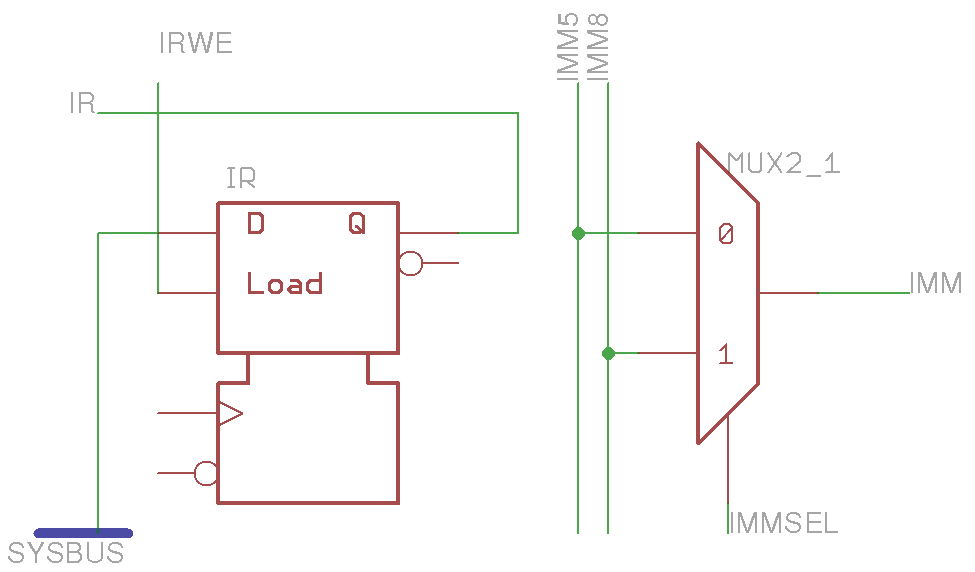
\includegraphics[width=0.4\textwidth]{../../eagle/Ir/IrAA.png}}
\subfloat[The BA type slice]{\label{fig:ir:circuit:ba}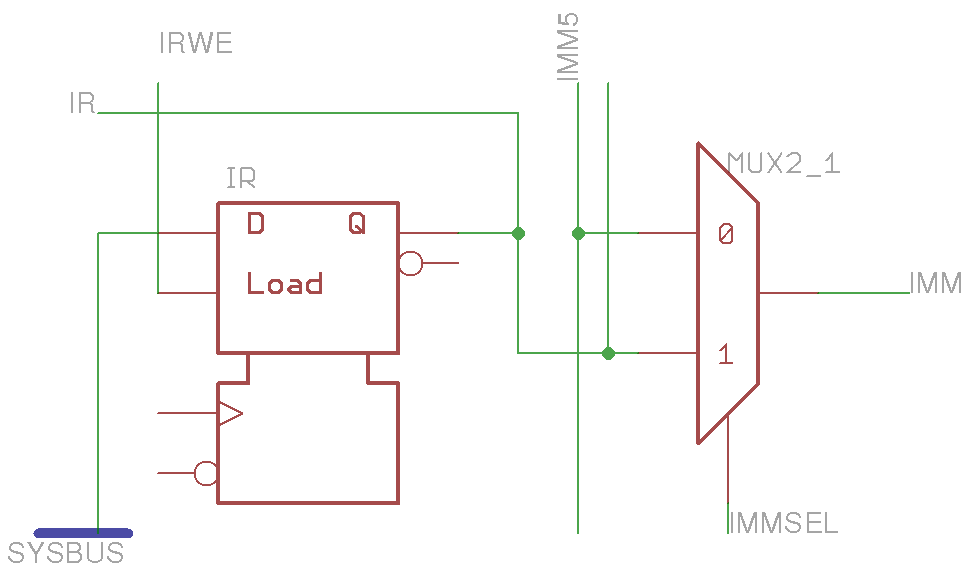
\includegraphics[width=0.4\textwidth]{../../eagle/Ir/IrBA.png}}\\
\subfloat[The BB type slice]{\label{fig:ir:circuit:bb}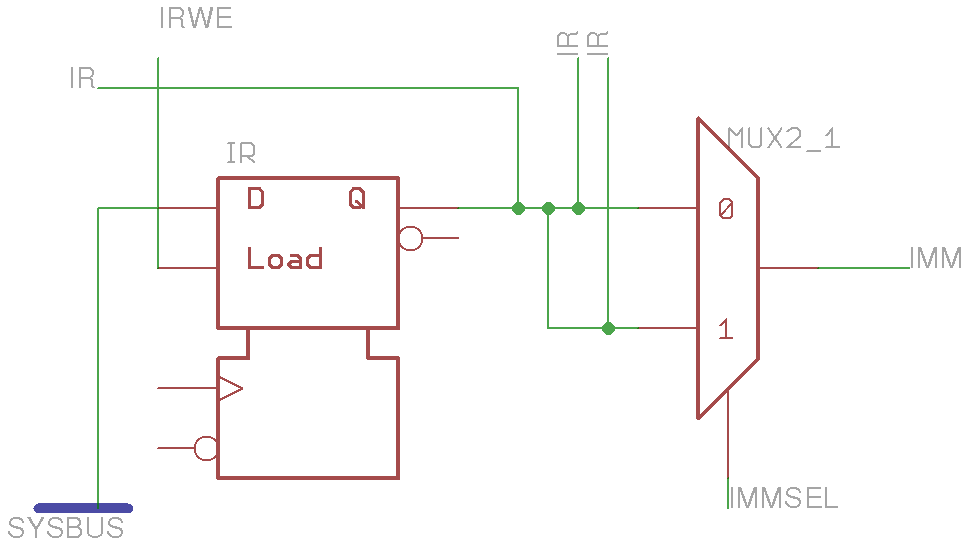
\includegraphics[width=0.4\textwidth]{../../eagle/Ir/IrBB.png}}
\caption{The three circuits used for the instruction register block.}
\label{fig:ir:circuit}
\end{figure}

